\documentclass[12pt,a4paper]{scrreprt}
 \usepackage{ngerman}
 \usepackage[utf8]{inputenc}

\usepackage{listings}


 \usepackage[T1]{fontenc}
\usepackage{pdfpages}
\usepackage{url}
\graphicspath{{/Users/Timo/Documents/DHBW/Semester4/Projektarbeit/}}
\usepackage{graphicx}
\usepackage{wrapfig}
\usepackage{geometry} 
\geometry{a4paper, top=25mm, left=25mm, right=25mm, bottom=25mm, headsep=15mm, 
  footskip=12mm}
\usepackage{textcomp}
% Header
\usepackage{fancyhdr}
\pagestyle{fancy}
% Header für Seiten ohne Chapter
\fancyhf{}
\fancyhead[L]{Studienarbeit Timo Höting \\ DHBW Karlsruhe}
   \fancyhead[R]{
\includegraphics[scale=0.3]{./data/dhbwlogo.jpg} } 
\fancyfoot[C]{\thepage}
\fancypagestyle{plain}{
% Header für Seiten mit Chapter
\fancyhf{}
   \fancyhead[L]{Studienarbeit Timo Höting \\ DHBW Karlsruhe}
   \fancyhead[R]{
\includegraphics[scale=0.3]{./data/dhbwlogo.jpg} } 
\fancyfoot[C]{\thepage}
}

\begin{document}
\begin{titlepage}
\begin{figure}
\makebox[\textwidth]{
\includegraphics[page={1},width=\paperwidth]{./data/deckblatt.pdf}} \\
\end{figure}
\end{titlepage}
\clearpage
\begin{figure}
\makebox[\textwidth]{
\includegraphics[page={2},width=\paperwidth]{./data/deckblatt.pdf}} \\
\end{figure}
\thispagestyle{empty} %Head löschen
\tableofcontents
\thispagestyle{empty}  
\chapter{Einleitung} 
\section{Einleitung}
Diese Studienarbeit wird im Zuge des Studiums Bachelor of Engineering - Informationstechnik an der DHBW Karlsruhe erstellt. \\\\
Im dieser Studienarbeit soll ein Komplettsystem entwickelt werden, dass sowohl die Über- wachung als auch die Steuerung der Beleuchtung von Innen- und Außenbereichen ermög- licht. Das System soll nach der Entwicklung universell einsetzbar und leicht konfigurierbar sein.\\\\
Die Beleuchtung soll mit adressierbaren LED-Pixeln umgesetzt werden, da diese sehr leicht steuer- und erweiterbar sind. Für die Erkennung von Bewegungen sollen klassische Bewegungsmelder eingesetzt werden. Mittels einer Kamera sollen Bilder aufgerufen und gespeichert werden können. Die gesamte Steuerung soll mittels einer iOS-App über einen Raspberry Pi möglich sein. Die Implementierung dieser App soll in Swift erfolgen und die der Server-Anwendung in Python.  \\\\
Es müssen passende Bauteile und Produkte evaluiert und getestet werden. Diese müssen vom Raspberry Pi ansteuerbar sein. Des weiteren muss die Architektur der Serveranwendung und iOS-App ausgearbeitet werden. Zur Fertigstellung müssen beide Anwendungen implementiert werden und die funktionsfähige Anwendung an einem Beispielobjekt in Betrieb genommen werden.\\\\
Es gibt drei verschiedene Modi in denen sich das System befinden kann:
\begin{itemize}
\item Beleuchtung wird durch Bewegungsmelder ausgelöst
\item Beleuchtung wird manuell vom Benutzer über App gesteuert 
\item Bewegungsmelder als Alarmanlage, beim Auslösen wird der Benutzer benachrichtigt und ein Bild der Kamera als Notifcation auf dem Smartphone angezeigt
\end{itemize}

\section{Teilprojekte}
\begin{itemize}
\item LED-Pixel und Bewegungssensoren evaluieren / ansteuern
\item Implementierung der Ansteuerung aller Bauteile
\item Implementierung der Netzwerkkommunikation
\item Implementierung der iOS App
\item praktische Umsetzung an einem Beispielobjekt
\end{itemize}

\section{Projektmanagement}
\subsection{Meilensteintrendanalyse}
Die Meilensteintrendanalyse ist eine Art des Projektmanagements. Hauptaufgabe ist die Überwachung des Projektfortschritts und die frühe Erkennung von Terminverzögerungen. Hierfür werden bei Projektbeginn Meilensteine festgelegt, die Inhalt, Dauer und Endzeitpunkt enthalten. Im Laufe eines Bearbeitungszeitraums können mögliche Verzögerungen erkannt und entsprechend darauf reagiert werden. Um große Verzögerungen zu vermeiden, sollten realistische Sicherheitspuffer eingeplant werden. \\
Bei Beendigung eines Meilensteins kann ein Fazit aus dessen Ablauf gezogen werden. Zum Beispiel kann bei aufgetretener Verzögerung Ursachenforschung betrieben werden, um in weiteren Schritten solche Verzögerungen zu vermeiden. 

\paragraph{Bemerkung}
\begin{itemize}
\item Die schriftliche Ausarbeitung ist nicht Teil der Meilensteine. Sie erfolgt parallel zu den durchgeführten Aufgaben.
\end{itemize}

\subsection{Meilensteine und Erfolgsprüfung}
\begin{enumerate}

\item Planung der Architektur (15. September - 30. September 2014)
\begin{itemize}
\item Entwurf Anwendungsstruktur
\begin{itemize}
\item Der Entwurf der Anwendungssturktur für Serverimplementierung und Mobile-Implementierung konnte erfolgreich abgeschlossen werden.
\end{itemize}
\item Ermittlung notwendiger Hardware für die einzelnen Anwendungsfälle
\begin{itemize}
\item Dies benötigte nur geringen Aufwand, da nur wenige Bauteile benötigt werden. Die Evaluierung, Beschaffung und Tests fällt in den 3. Meilenstein.
\end{itemize}
\item Ausarbeitung Übertragungsprotokoll
\begin{itemize}
\item Das Protokoll wurde erfolgreich ausgearbeitet. Die Details sind in 2.5.1 dargestellt.
\end{itemize}
\item Einarbeitung in Python
\begin{itemize}
\item Es wurden die Grundlagen der Sprache Python im Bezug auf OOP, Funktionen und Datentypen erarbeitet. Die Kenntnisse haben sich im Laufe des Projekts weiter verbessert. 
\end{itemize}
\end{itemize}

\item Funktionsfähiger Prototyp Webserver (1. Oktober - 19. Oktober 2014)
\begin{itemize}
\item Auswahl eines Frameworks für die Implementierung des Webservers
\begin{itemize}
\item Es wurde das Twisted Framework ausgewählt und Testimplementierung der verschiedenen Server-Typen (Socket, SSL, STARTTLS, HTTP, HTTPS) durchgeführt. 
\end{itemize}
\item Implementierung der für den Webserver nötigen Klassen
\begin{itemize}
\item Implementierung der Socketübertragung. Im Laufe des Projekts zeigte sich, dass dies nicht die optimale Lösung ist. in einem späteren Meilenstein wurde ein HTTPS-Webserver mit Twisted implementiert. 
\end{itemize}
\item Testen der Funktionen
\begin{itemize}
\item Testen mithilfe von Clients, die in Python implementiert wurden. 
\end{itemize}
\end{itemize}

\item Auswahl Hardwarekomponenten (LEDs, Sensoren, Kamera) (20. Oktober - 31. Oktober 2014)
\begin{itemize}
\item Evaluierung
\begin{itemize}
\item Die Evaluierung von LEDs und Sensoren konnte erfolgreich abgeschlossen werden. Für die Wahl der Netzwerkkamera konnte keine Lösung gefunden werden, da noch nicht klar war, in welcher Form die Bilder abgerufen werden können. Dieser Aufgabenteil ist in Meilenstein 7 verschoben worden.
\end{itemize} 
\item Beschaffung
\begin{itemize}
\item Die Beschaffung von LEDs und Sensoren verlief mit erfolgreich mit geringem Aufwand. 
\end{itemize}
\item Testen und Testimplementierung
\begin{itemize}
\item Die Testimplementierungen erfolgreich durchgeführt werden. Der Quellcode und die zugehörigen Schaltbilder befinden sich in den Punkten 2.1 und 2.2.
\end{itemize}
\end{itemize}

\item Implementierung Serveranwendung (1. November - 30. November 2014)
\begin{itemize}
\item Implementierung Sensorerkennung
\begin{itemize}
\item Die Implementierung der Sensorerkennung war erfolgreich.
\end{itemize}
\item Implementierung Ansteuerung LED
\begin{itemize}
\item Die Implementierung der Ansteuerung der LEDs war erfolgreich.
\end{itemize}
\item Implementierung der Konfigurationsmöglichkeiten ( hat nicht geklappt -> Dezember, Januar)
\begin{itemize}
\item Die vollständige Implementierung der Konfigurationsdateien, -lesern und -schreibern, sowie der Übertragung wurde nicht abgeschlossen. Grund dafür war fehlende Kenntniss über den Empfang auf dem Client und über JSON.
\end{itemize}
\item Implementierung des Übertragungsprotokolls
\begin{itemize}
\item Die Auswertung der empfangenen Daten wurde erfolgreich implementiert. 
\end{itemize}
\item Komplette Implementierung 
\begin{itemize}
\item Die Implementierung der gesamten Serveranwendung wurde soweit fertiggestellt, dass ein Betrieb möglich war. Einige kleine Änderungen oder nachträgliche Erweiterungen wurden im Laufe des Projekts hinzugefügt. Dies waren meistens Dinge, die vorher nicht bedacht wurden, oder an die mobile App angepasst werden mussten.
\end{itemize}
\end{itemize}

\item Funktionsfähiger Prototyp iOS-Anwendung (1. Januar - 31. Januar 2015)
\begin{itemize}
\item Einarbeitung Swift und XCode
\begin{itemize}
\item In dieser Zeitphase wurde der Umgang mit XCode und der Sprache Swift erlernt. 
\end{itemize}
\item Erstellung Prototyp der Anwendung in XCode
\begin{itemize}
\item Es wurde die Anwendungsstrktur in XCode erstellt. 
\end{itemize}
\item Auswahl von nötigen Frameworks
\begin{itemize}
\item Es wurden Frameworks für Menüführung, Sicherheit und FTP-Verbindung ausgewählt und hinzugefügt. 
\end{itemize}
\item Übertragungen mit dem Webserver
\begin{itemize}
\item In dieser Phase wurde festgestellt, dass die Übertragung über Sockets nicht optimal ist. Eine Übertragung mittels HTTP Protokoll bietet eine deutlich einfachere und sicherere Implementierung. Aufgrund dieser Feststellung wurde die Implementierung des Webservers in diesem Meilenstein verändert. 
\end{itemize}
\item Refactoring Webserver
\begin{itemize}
\item Der Webserver wurde auf HTTPS umgestellt. 
\item Viele kleine Veränderungen im Server.
\end{itemize}
\end{itemize}

\item Implementierung iOS-Anwendung (1. Februar - 31. März 2015)
\begin{itemize}
\item Server-Client Kommunikation
\begin{itemize}
\item Die Übertragung wurde entsprechend dem Anwendungsprotokoll implementiert. 
\end{itemize}
\item User-Interface
\begin{itemize}
\item Das User-Interface wurde erstellt und mit Funktionen versehen. 
\end{itemize}
\item Implementierung konsistene Speicherung
\begin{itemize}
\item Der Zugriff auf CoreData wude implementiert.
\end{itemize}
\end{itemize}

\item Abschluss der Arbeit (1. April - 11. Mai 2015)
\begin{itemize}
\item Implementierung Netzwerkkamera
\begin{itemize}
\item Die Anbindung der Netzwerkkamera war einer der aufwändigsten Punkte in diesem Projekt. Nach verschiedenen Ansätzen wurde eine gute Lösung erarbeitet.
\end{itemize}
\item Beispielobjekt
\begin{itemize}
	\item Das gesamte Projekt wurde in einem Treppenhaus installiert.
\end{itemize}
\item Fertigstellung Ausarbeitung
\item  Abgabe
\end{itemize}

\end{enumerate}


\chapter{Hauptteil}
\section{LED-Pixel} 
\subsection{Bewertungskriterien}
Die Beleuchtung soll durch einzelne LED-Pixel stattfinden. Ein Pixel bedeutet ein Chip auf dem sowohl die LED und der nötige Treiber sitzt. Für die Evaluierung werden folgende Kriterien gewählt:
\begin{itemize}
\item RGB-Farbraum \\
Die LED muss den gesamten RGB-Farbraum darstellen können. \\
Gewichtung: 5, KO-Kriterium
\item Ansteuerung \\
Da der Raspberry Pi an einigen seiner Pins Pulsweitenmodulation\footnote{Pulsweitenmodulation: Signalübertragung durch Wechsel zwischen zwei Spannungen (High, Low), Breite des Impulses ist das Signal} (PWM) bietet, sollten die LED-Pixel ohne extra Hardware ansteuerbar sein. Eine extra Stromversorgung ist aber bei größerer Anzahl an LEDs unabdingbar. \\
Gewichtung: 10
\item Framework \\
Hier wird bewertet ob der jeweilige Hersteller ein fertiges Framework zu seinen Produkten anbietet. \\
Gewichtung: 10
\item Kosten \\
Es werden nur die reinen Produktkosten, also ohne Versand und Zoll, bewertet. \\
Gewichtung: 5
\item Extras \\
An dieser Stelle können mögliche Extras eines Herstellers einfließen. \\
Gewichtung: 5
\end{itemize}

\subsection{Evaluierung}
\begin{itemize}
\item Adafruit, Neopixel \\
https://www.adafruit.com/neopixel \\
LED-Pixel in unzähligen Ausführungen. \\
Sitz der Firma in Tampa, Florida, USA \\
RGB: Chip ist der WS2801, http://www.adafruit.com/datasheets/WS2801.pdf -> Hat volle Abdeckung des RGB-Farbraums \\
Ansteuerung: Findet über PWM-Pin des Raspberry Pi statt. \\
Framework: Framework von Adafruit, welches eine sehr leichte Ansteuerung ermöglichen soll. \\
Kosten: 4 LEDs  7\$, 25 LEDs zusammen  39\$, durch Lieferung aus USA sehr hohe Versandkosten (50\$) \\
Extras: Händler bietet verschiedene Formen und fertige Ketten an. \\
\item LED-Emotion GMBH, LED Streifen \\
http://www.led-emotion.de/de/LED-Streifen-Set.html \\
LED-Streifen, keine Einzelpixel, nur mit Controller, keine API \\
RGB: Voller RGB-Farbraum \\
Ansteuerung: Nur mit Controller  \\
Framework: Keine öffentliche Api, möglicherweise mit Raspberry Pi ansteuerbar  \\
Kosten: 30 LEDs mit Netzteil 79€   \\
Extras: keine
\item DMX4ALL GmbH, MagiarLED Solutions \\
http://www.dmx4all.de/magiar.html \\
Spezialisiert auf DMX-Ansteuerung, keine öffentliche API \\
RGB: Volle Abdeckung RGB-Farbraum \\
Ansteuerung: Wird über DMX-Controller angesteuert, dieser setzt die Signale um. \\
Framework: DMX-Ansteurung über DMX-Controller \\
Kosten: Streifen mit 72 LEDs = 99€ \\
Extras: viele verschiedene Varianten
\item TinkerForge, RGB LED-Pixel \\
https://www.tinkerforge.com/de/shop/accessories/leds.html \\
Scheinen die gleichen wie von Adafruit zu sein, allerdings werden hauptsächlich Controller im Shop angeboten \\
RGB: Chip WS2801, volle Abdeckung RGB-Farbraum \\
Ansteuerung: Nach Anfrage an den Anbieter sollen die LEDs baugleich zu denen von Adafruit sein.  \\
Framework: keins, aber Ansteuerung über das Framework von Adafruit \\
Kosten: 50 LEDs = 59€ \\
Extras: Lieferung aus Deutschland
\end{itemize}
\begin{minipage}{\linewidth}
            \centering
            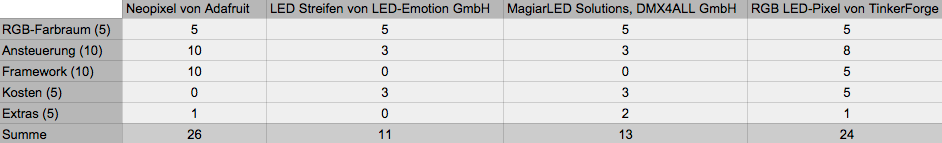
\includegraphics[width=\textwidth]{./data/evaluierung-led.png}
            \captionof{figure}{Ergebnisse der LED-Evaluierung}
        \end{minipage}
\paragraph{Fazit:}
In der Evaluierung schneiden die Produkte von Adafruit und TinkerForge am besten ab. Für eine erste Teststellung werden die einzelnen LED-Pixel von Adafruit aus den USA bestellt (Neopixel). An diesen soll vor allem die Ansteuerung getestet werden. Falls sie sich bewähren, wird für den endgültigen Aufbau auf die LED-Ketten von Tinkerforge zurück gegriffen. 

\subsection{Teststellung}
Für einen ersten Test wurde das in XXX ausgewählte Produkt als einzelne Pixel bestellt. Der Hersteller Adafruit bietet hier 4er-Packungen an. Diese können leicht in eigene Schaltungen eingelötet oder auf Experimentier-Boards gesteckt werden. Bei geringer Anzahl LEDs reicht die 5V-Stromversorgung des Raspberry Pi aus. 
\paragraph{Technische Daten Neopixel:} 
	\begin{itemize}
	\item Maße: 10.2mm x 12.7mm x 2.5mm
	\item Protokollgeschwindigkeit: 800 kHz
	\item Spannung: 5-9VDC  (bei 3,5V gedimmte Helligkeit) 
	\item Strom: 18,5mA / LED, 55mA / Pixel
	\end{itemize}
\paragraph{Framework:}
	\begin{itemize}
	\item RPI\_WS281X (https://github.com/jgarff/rpi\_ws281x)
	\item Sprache: Python
	\item Entwickelt für Raspberry Pi
	\item Vorraussetzung: Python 2.7
	\end{itemize}
\paragraph{Ablauf des Tests:}
\begin{itemize}

\item \textbf{Aufbau der Schaltung}\\
An die einzelnen LED-Pixel wurden Stecker angelötet, damit sie auf das Experimentierboard aufgesteckt werden können. Dann wird die Schaltung nach folgendem Schaltbild verbunden. Wichtig ist, dass beim Raspberry Pi nur Pins verwendet werden können, welche PWM bieten. \\
\begin{minipage}{\linewidth}
            \centering
            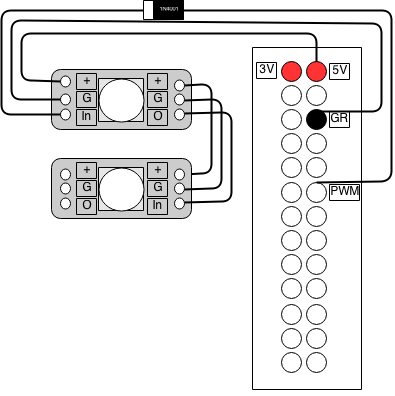
\includegraphics[width=8cm]{./data/TestSchaltungLED.png}
            \captionof{figure}{Schaltung für LED-Test}
        \end{minipage}
\item \textbf{Installation des Frameworks} 
\begin{lstlisting}[caption = Installation Framework ws281x, language=Python, frame=single, breaklines=true,columns=fullflexible, commentstyle=\color{gray}\upshape, captionpos=b, numbers = left]
wget https://github.com/tdicola/rpi_ws281x/raw/master/python/dist/rpi_ws281x-1.0.0-py2.7-linux-armv6l.egg 
sudo easy_install rpi_ws281x-1.0.0-py2.7-linux-armv6l.egg
\end{lstlisting}
\item \textbf{Testcode}

\begin{lstlisting}[caption = Testcode zur Ansteuerung der LEDs, language=python, frame=single, breaklines=true,columns=fullflexible, commentstyle=\color{gray}\upshape, captionpos=b, numbers = left]
from neopixel import * 
	
LED_COUNT   = 4       # Number of LED pixels. 
LED_PIN     = 18      # GPIO pin connected to the pixels (must support PWM!).
LED_FREQ_HZ = 800000  # LED signal frequency in hertz (usually 800khz)
LED_DMA     = 5       # DMA channel to use for generating signal (try 5)
LED_INVERT  = False   # True to invert the signal (when using NPN)

strip = Adafruit_NeoPixel(LED_COUNT, LED_PIN, LED_FREQ_HZ, LED_DMA, LED_INVERT)

strip.begin()
strip.setPixelColor(0, Color(255, 255, 255))
strip.setPixelColor(1, Color(255, 255, 255))
strip.setPixelColor(2, Color(255, 255, 255))
strip.setPixelColor(3, Color(255, 255, 255))
strip.show()
\end{lstlisting}
\end{itemize}
\paragraph{Fazit}
Die einzelnen Pixel sind sehr leicht anzusteuern, unterstützen auch das automatische Abschalten nach einer bestimmten Zeit und haben eine sehr hohe Leuchtkraft. Die Evaluierung hat zu einer guten Produktwahl geführt. \\ 
Nach einer weiteren Nachfrage an Tinkerforge wurde versichert, dass deren LED-Ketten Baugleich zu denen von Adafruit sind. Aufgrund der hohen Versandkosten werden für die endgültige Teststellung die Produkte von Tinkerforge gewählt.

\section{Bewegungssensor} In einem der Modi soll die Beleuchtung durch den Bewegunsmelder ausgelöst werden. Hierfür sind zuverlässige und weitreichende Bewegungssensoren notwendig.
\subsection{Bewertungskriterien}
\begin{itemize}
\item \textbf{Ansteuerung}\\
Die Anbindung an den Raspberry Pi soll möglichst leicht realisierbar sein. Wünschenswert ist, dass der Sensor einfach ein High-Signal bei Bewegungserkennung ausgibt. \\
Gewichtung: 5, KO-Kriterium
\item \textbf{Reichweite}\\
Die Reichweite oder Sensivität des Sensors soll ausreichend und regelbar sein.\\
Gewichtung: 3
\item \textbf{Kosten}\\
Es werden nur die reinen Produktkosten, also ohne Versand und Zoll, bewertet. \\
Gewichtung: 1
\item \textbf{Extras}\\
An dieser Stelle können mögliche Extras eines Herstellers einfließen.\\
Gewichtung: 3
\end{itemize}

\subsection{Evaluierung}
\begin{itemize}
\item \textbf{PIR (MOTION) Sensor, Adafruit}\\
Link: \url{http://www.adafruit.com/product/189}\\
Ansteuerung: Gibt High-Signal an einem Pin aus.\\
Reichweite: 7m, 120 Grad\\
Kosten: 9,95\$ + Versand aus USA\\
Extras: Kabel inklusive\\
\item \textbf{PIR Infrared Motion Sensor (HC-SR501)}\\
Link: \url{https://www.modmypi.com/pir-motion-sensor}\\
Ansteuerung: Gibt High-Signal an einem Pin aus.\\
Reichweite: 5-7m, 100 Grad\\
Kosten: 2,99\$ + Versand aus UK\\
Extras: keine\\
\item \textbf{Infrarot PIR Bewegung Sensor Detektor Modul}\\
Link: \url{http://www.amazon.de/Pyroelectrische-Infrarot-Bewegung-Sensor-Detektor/dp/B008AESDSY/ref=pd\_cp\_ce\_0}\\
Ansteuerung: Gibt High-Signal an einem Pin aus.\\
Reichweite: 7m, 100 Grad\\
Kosten: 5 Stück = 7,66€\\
Extras: keine\\
\end{itemize}
\begin{figure}[h]
\begin{minipage}{\textwidth}
            \centering
            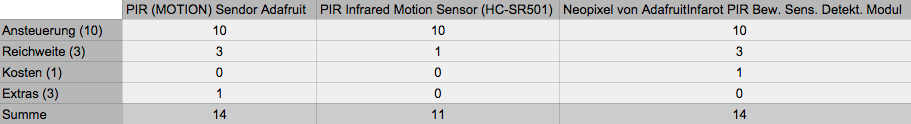
\includegraphics[width=\textwidth]{./data/evaluierung-ms.png}
            \caption{Ergebnisse der Motion-Sensor-Evaluierung}
        \end{minipage}
\end{figure}
\paragraph{Fazit}
Die meisten Infarot-Bewegungssensoren sind von der Bauweise nahezu identisch. Die Unterschiede liegen meist nur in der Empfindlichkeit. Da die Reichweite in diesem Fall nicht von großer Bedeutsamkeit ist, kann eigentlich jedes der Produkte bestellt werden. Auf Ebay und Amazon ist die Anzahl angebotener Sensoren nahezu unbegrenzt, es wurde für die Teststellung also die oben evaluierte Variante von Amazon bestellt. 
\subsection{Teststellung}
Der in Punkt X.X.X gewählte Bewegungssensor wurde beim Hersteller bestellt. In der Teststellung reicht die Stromversorgung des Raspberry Pi. 
\paragraph{Technische Daten Sensor:}
\begin{itemize}
\item Die Empfindlichkeit und Haltezeit kann eingestellt werden
\item Reichweite: ca. 7m
\item Winkel: 100 Grad
\item Spannung: DC 4,5V- 20V
\item Strom: < 50uA
\item Ausgansspannung: High 3V / Low 0V
\item Größe: ca. 32mm x 24mm
\end{itemize}

\paragraph{Ablauf des Tests:}
\begin{itemize}
\item \textbf{Aufbau der Schaltung} \\
Der Sensor wird in der Teststellung direkt vom Raspberry Pi mit Strom versorgt. Für die Datenleitung kann jeder beliebige Pin gewählt werden. 
\item \textbf{Testcode} \\
Um eine Änderung am Datenpin festzustellen werden zwei Variable angelegt: current\_status und previous\_status. Das Programm wird in einer Dauerschleife geschickt, in der bei jedem Durchlauf die beiden Status überprüft. Wenn der neue Status (current\_status) High ist und das vorherige Signal (previous\_state) Low, dann wird eine Bewegung erkannt. Der Code wird mittels Kommentare erklärt.	

\begin{lstlisting}[caption = Testcode zur Bewegungserkennung mit Sensor, language=python, frame=single, breaklines=true,columns=fullflexible, commentstyle=\color{gray}\upshape, captionpos=b, numbers = left]
import RPi.GPIO as GPIO
import time
GPIO.setmode(GPIO.BCM)
# Pin definieren
MOTION_PIN1 = 7
# Diese als Input definieren
GPIO.setup(MOTION_PIN1,GPIO.IN)
# Status definieren um verschiedene Änderungen zu erkennen
Current_State  = 0
Previous_State = 0

try:
	# Loop zur Erkennung einer Bewegung
	# Sensor erkennt Bewegung -> Signal = High
	# Wartet 3 Sekunden und setzt Signal = Low
	while True :
		Current_State = GPIO.input(MOTION_PIN1)
		if Current_State == 1 and Previous_State == 0:
			print "Motion detected!"
			Previous_State=1
		elif Current_State == 0 and Previous_State == 1:
			print "Ready"
			Previous_State=0
		time.sleep(0.01)
	
except KeyboardInterrupt:
	print "Quit"
	GPIO.cleanup()
\end{lstlisting}
Bei der Endversion des Systems sollen mehrere Beweungssensoren integriert werden. Bei Auslösen des ersten Sensors sollen die LEDs angeschaltet werden und nach auslösen eines weiteren Sensors wieder ausgeschaltet werden.  
\end{itemize}

\paragraph{Auswertung}
Das High-Signal des Sensors lässt sich mit dem Raspberry Pi sehr leicht auswerten. Auch die Auswertung von mehreren Sensoren stellt kein Problem da. Das Ergebnis der Evaluierung konnte in dieser Teststellung bestätigt werden. Wichtig für die weitere Implementierung ist, dass die While-Schleife auch abgebrochen werden kann. 


\section{Verschlüsselung}

\subsection{SSL vs. TLS}
SSL (Secure Sockets Layer) und TLS (Transport Layer Security) sind Protokolle, die Verschlüsselung und Authentifizierung zwischen zwei Kommunikationspartnern bieten. Die beiden Begriffe SSL und TLS werden umgangssprachlich oft als zwei verschiedene Techniken dargestellt, obwohl TLS eine Weiterentwicklung von SSL ist. SSL v3 ist die Basis von TLS 1.0. \\
Aufgrund des Alters und einiger Sicherheitslücken wird SSL als unsicher angesehen und soll nicht mehr verwendet werden. Die aktuellste gefundene Lücke ist POODLE\footnote{SIcherheitslücke in SSL v3}, welche das Auslesen von Informationen aus einer verschlüsselten Übertragung erlaubt. Die Weiterentwicklungen TLS 1.1 und 1.2 sind deutlich sicherer und beheben einige Sicherheitslücken. So schützt die richtige Implementierung von TLS 1.2 auch vor den BEAST\footnote{Sicherheitslücke in TLS v1.0} Angriffsmethoden.\\

\subsection{Vor- und Nachteile TLS}
Da TLS auf der Transportschicht aufsetzt kann jedes höhere Protokoll darüber übertragen werden, somit ist die Verschlüsselung unabhängig von der genutzten Anwendung. \\
	Der größte Nachteil besteht darin, dass der Verbindungsaufbau serverseitig sehr rechenintensiv ist. Die Verschlüsselung selbst nimmt, abhängig vom Algorithmus, nur noch wenig Rechenleistung in Anspruch. \\

\subsection{TLS Handshake}
1. Client Hello\\
Übertragung von Verschlüsselungsinformationen vom Client an den Server, wie TLS Version oder Verschlüsselungsmöglichkeiten\\
2. Server Hello \\
Server sendet seine Informationen und legt Verschlüsselung fest. \\
3. Server Key Exchange\\
Server sendet seine Identität in Form seines Zertifikats. \\
4. Client Key Exchange\\
Client legt seinen Pre-Shared-Key fest und überträgt ihn verschlüsselt mit dem public Key des Servers.\\
5. Change Cipher Spec\\
Aus dem PSK wird ein Master-Secret generiert, mit welchem die folgenden Übertragung abgesichert wird. \\
6. Application Data\\
Übertragung der Daten. \\

\subsection{StartTLS}
Eine Variante von TLS ist das sogenannte STARTTLS, bei dem zuerst ein unsicheres 'hello' an den Server gesendet wird. Falls im Anschluss eine Verbindung erfolgreich Zustande kommt, wird zur sicheren Übertragung gewechselt. \\
Im ersten Versuch der Server-Client-Kommunikation in diesem Projekt wurden die Daten direkt zwischen Sockets übertragen. Im folgenden Ausschnitt ist der Wechsel zur Verschlüsselung sehr gut erkennbar: 
\begin{lstlisting}[caption = Starttls - Wechsel zur Verschlüsselung, language=python, frame=single, breaklines=true,columns=fullflexible, commentstyle=\color{gray}\upshape, captionpos=b, numbers = left]
if line == "STARTTLS":
	print "-- Switching to TLS"
	self.sendLine('READY')
	ctx = ServerTLSContext(
		privateKeyFileName='./certs/server.key',
		certificateFileName='./certs/server.crt',
			)
	self.transport.startTLS(ctx, self.factory)
\end{lstlisting}
Der vollständige Code ist im Commit unter \url{https://github.com/hoedding/Studienarbeit-Anwendung/commit/b52d056f55a9d65b9115ead2d2a2c0a549b366b6} zu finden

\subsection{Server Zertifikat}
Für die Verschlüsselung der Übertragung zwischen Server und Client ist ein Server-Zertifikat notwendig. Dieses wird mit OpenSSL in der neuesten Version generiert. \\
1. Private Key erzeugen
\begin{lstlisting}[caption =private Key, language=python, frame=single, breaklines=true,columns=fullflexible, commentstyle=\color{gray}\upshape, captionpos=b, numbers = left]
openssl genrsa -des3 -out server.key 2048
\end{lstlisting}

2. Certificate Signing Request
\begin{lstlisting}[caption =Certificate Signing Request, language=python, frame=single, breaklines=true,columns=fullflexible, commentstyle=\color{gray}\upshape, captionpos=b]
openssl req -new -key server.key -out server.csr
\end{lstlisting}


3. Self Signed Certificate\\
Bei einem öffentlichen Server sollte das Zertifikat bei einer CA (Certificate Authority) signiert werden. \\
\begin{lstlisting}[caption =Self Signed Certificate, language=python, frame=single, breaklines=true,columns=fullflexible, commentstyle=\color{gray}\upshape, captionpos=b]
openssl x509 -req -days 1865 -in server.csr -signkey server.key -out server.crt
\end{lstlisting}

\subsection{Apple Zertifikat}
Um die Apple Push Notifications einzusetzen ist ein Apple-Developer Zertifikat notwendig, welches nur über das Apple-Developer Portal erzeugt werden kann. Hierfür muss eine App-Identität angelegt werden. Im Anschluss wird auf einem Apple-Gerät ein Signing-Request erstellt. Dieser wird in das Developer-Portal hochgeladen. Im Anschluss wird ein Zertifikat generiert. Dieses muss in das Verzeichnis 'certs' gelegt werden. \\
Zusätzlich ist auf dem System ein Apple-Root Zertifikat erforderlich.\\\\
Die Generierung von Zertifikaten im Developer-Portal ist nur mit gültiger Apple-Developer-Registrierung möglich.

\subsection{Wireshark Trace}
Im folgenden ist ein Trace eines TLS Handshakes zwischen einem Client und dem implementierten Server (mit Twisted Framework) auf dem Raspberry Pi zu sehen. \\
Die einzelnen Schritte des Handshakes sind sehr gut erkennbar.\\
\begin{figure}[h]
\begin{minipage}{\textwidth}
            \centering
            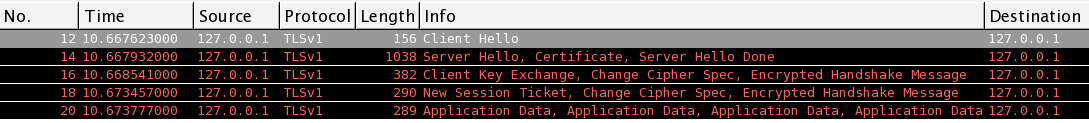
\includegraphics[width=\textwidth]{./data/wireshark.png}
            \caption{Wireshark Trace TLS Handshake}
        \end{minipage}
\end{figure}
\section{Python-Server und Protokoll} 
\subsection{Protokoll}
Um die LEDs später von einer App aus ansprechen zu können, soll ein auf Strings basierendes Protokoll implementiert werden. Dieses wird in TCP-Paketen übertragen. Hierfür muss als erstes festgelegt werden, welche Informationen übertragen werden sollen: \\
\begin{itemize}
\item Authentifizierung\\
Übertragung eines Passworts. Dieses ist als Hashwert im System gespeichert und kann so überprüft werden. Es wird der SHA-224-Algorithmus eingesetzt.
\item Control\\
Unterscheidung zwischen:\\
	X00: Alle LEDs ausschalten\\
	X01: Eine LED anschalten\\
	X02: LED-Bereich anschalten\\
	X03: Effekt für eine LED\\
	X04: Effekt für LED-Bereich\\
	X05: Effektcode \\\\
Abhängig von diesem Feld werden die nachfolgenden Werte behandelt. 
\item LED-Nummer\\
Falls nur eine LED angesprochen werden soll (Control = X00), so wird hier die Nummer angegeben. Ob sie im gültigen Range liegt wird intern überprüft.
\item Bereich Start\\
Wenn mehrere LEDs gesteuert werden sollen (Control = X01), so wird hier der Beginn des Bereichs angegeben.
\item Bereich Ende\\
Und hier das Ende des Bereichs. 
\item Rot\\
Farbwert Rot 0-255
\item Grün\\
Farbwert Grün 0-255
\item Blau\\
Farbwert Blau 0-255
\item Effekt\\
Es können verschiedene LEDs mit Effekten belegt werden, wie zum Beispiel Aufblitzen oder zeitgesteuertes Ausschalten.
\item Effektcode\\
Hinterlegte, fest programmierte Effekte, zum Beispiel alle LEDs anschalten in weis mit höchster Leuchstärke.
\item Hash\\
Überprüfung ob die Übertragung erfolgreich war, mittels eines Hashwertes. Es wird der SHA-224-Algorithmus eingesetzt.
\end{itemize}
\textbf{Übertragungsbeispiel:}\\
		Protokoll: 	
\begin{lstlisting}[caption = Beispielübertragung des Protokolls, language=python, frame=single, breaklines=true,columns=fullflexible, commentstyle=\color{gray}\upshape, captionpos=b]
auth:control:ledNo:rangeStart:rangeEnd:red:green:blue:effect:effectcode:hash
pass:X01:0:0:49:255:255:255:0:0:xx
Dies würde die LEDs 0 bis 49 einschalten (Farbe weis 255,255,255)
\end{lstlisting}
\subsection{Framework}
Twisted: https://twistedmatrix.com \\
Es wird das Twisted Matrix Framework eingesetzt. Twisted ist eine in Python geschriebene  event-getriebene Netzwerkengine. Die meisten gängigen Protokolle wie TCP, IMAP, SSHv3 und viele mehr werden unterstützt. Somit bietet Twisted die ideale Möglichkeit einen eigenen simplen Server zu implementieren. \\\\
\textbf{Event-Getrieben (event-based):} Die Serveranwendung befindet sich in einer Schleife und wartet auf ein Event. Dieses Event ist in diesem Fall der Connect eines Clients zum Server. Für jeden Connect wird eine neue Instanz angelegt, in welcher empfangene Daten bearbeitet werden können. 

\subsection{Testcode}
\begin{lstlisting}[caption =Testcode Echoserver mit Twisted Framework, language=python, frame=single, breaklines=true,columns=fullflexible, commentstyle=\color{gray}\upshape, captionpos=b, numbers = left]
#!/usr/bin/env python
# Copyright (c) Twisted Matrix Laboratories.
# See LICENSE for details.

from twisted.internet.protocol import Protocol, Factory
from twisted.internet import reactor

### Protocol Implementation

# This is just about the simplest possible protocol
class Echo(Protocol):
	def dataReceived(self, data):
		self.transport.write(data)


	def main():
		f = Factory()
		f.protocol = Echo
		reactor.listenTCP(8000, f)
		reactor.run()

if __name__ == '__main__':
main()
\end{lstlisting}

//TODO ERKLÄRUNG

\subsection{Implementierung}
Im Folgenden wird die Implementierung des Servers näher erläutert. \\\\
	
	// TODO CODE des Servers

\subsection{Klassen und ihre Funktionen}
// TODO
\subsection{Hashfunktion}
Es wird zu zweierlei Zwecken eine Hashfunktion eingesetzt. Zum einen um die Korrektheit der Übertragung zu überprüfen und zum Anderen um ein Passwort zur Authentifizierung verwenden zu können. Dieses wird als Wort übertragen, auf dem Server aber nur als Hash-Wert abgespeichert. Falls es also jemand schafft die Konfirgurationsdatei abzugreifen, so ist der Passworthash nichts wert. 

\section{Verschlüsselung}
\subsection{SSL vs. TLS}
SSL (Secure Sockets Layer) und TLS (Transport Layer Security) sind Protokolle, die Verschlüsselung und Authentifizierung zwischen zwei Kommunikationspartnern bieten. Die beiden Begriffe SSL und TLS werden umgangssprachlich oft als zwei verschiedene Techniken dargestellt, obwohl TLS nur eine Weiterentwicklung von SSL ist. SSL v3 ist die Basis von TLS 1.0. \\
Aufgrund des Alters und einiger Sicherheitslücken wird SSL als unsicher angesehen und soll nicht mehr verwendet werden. Die aktuellste gefundene Lücke ist POODLE, welche das Auslesen von Informationen aus einer verschlüsselten Übertragung erlaubt. Die Weiterentwicklungen TLS 1.1 und 1.2 sind deutlich sicherer und beheben einige sicherheitslücken. \\
Eine Variante von TLS ist das sogenannte STARTTLS, bei dem zuerst ein unsicheres 'hello' an den Server gesendet wird. Falls im Anschluss eine Verbindung erfolgreich Zustande kommt, wird zur sicheren Übertragung gewechselt. \\
Wenn ein Server implementiert wird, so muss er alle Techniken unterstützen, beim Client kann der Entwickler selbst entscheiden. Ein Entwickler sollte immer die höchsten Verschlüsselungstechniken einsetzen. \\

\subsection{Vor- und Nachteile TLS}
Jedes höhrer Protokoll kann über TLS übertragen werden, somit ist die Verschlüsselung unabhängig von der genutzten Anwendung. \\
	Der größte Nachteil besteht darin, dass der Verbindungsaufbau serverseitig sehr rechenintensiv ist. Die Verschlüsselung selbst nimmt, abhängig vom Algorithmus, nur noch wenige Rechenleistung in Anspruch. \\

\subsection{TLS Handshake}
1. Client Hello\\
Übertragung von Verschlüsselungsinformationen vom Client an den Server, wie TLS Version oder Verschlüsselungsmöglichkeiten\\
2. Server Hello \\
Server sendet seine Informationen und legt Verschlüsselung fest. \\
3. Server Key Exchange\\
Server sendet seine Identität in Form seines Zertifikats. \\
4. Client Key Exchange\\
Client legt seinen Pre-Shared-Key fest und überträgt ihn verschlüsselt mit dem public Key des Servers.\\
5. Change Cipher Spec\\
Aus dem PSK wird ein Master-Secret generiert, mit welchem die folgenden Übertragung abgesichert wird. \\
6. Application Data\\
Übertragung der Daten. \\

\subsection{Zertifikat und Key}
Auf dem Raspberry Pi ist OpenSSL in der neuesten Version installiert. Es wird ein selbst-signiertes Zertifikat im 2048 Bit Key erzeugt.\\
1. Private Key erzeugen\\
openssl genrsa -des3 -out server.key 2048\\
2. Certificate Signing Request\\
openssl req -new -key server.key -out server.csr\\
3. Self Signed Certificate\\
Bei einem öffentlichen Server sollte das Zertifikat bei einer CA (Certificate Authority) signiert werden. \\
openssl x509 -req -days 1865 -in server.csr -signkey server.key -out server.crt

\subsection{Beispielcode STARTTLS Server}
An dieser Stelle ist der Beispielcode von Twisted am besten verständlich\\
(Quelle: https://twistedmatrix.com/documents/12.3.0/core/howto/ssl.html)\\
\begin{lstlisting}[caption =Testcode Echoserver mit Twisted Framework, language=python, frame=single, breaklines=true,columns=fullflexible, commentstyle=\color{gray}\upshape, captionpos=b, numbers = left]
from OpenSSL import SSL
from twisted.internet import reactor, ssl
from twisted.internet.protocol import ServerFactory
from twisted.protocols.basic import LineReceiver

class TLSServer(LineReceiver):
    def lineReceived(self, line):
        print "received: " + line

        if line == "STARTTLS":
            print "-- Switching to TLS"
            self.sendLine('READY')
            ctx = ServerTLSContext(
                privateKeyFileName='keys/server.key',
                certificateFileName='keys/server.crt',
                )
            self.transport.startTLS(ctx, self.factory)


class ServerTLSContext(ssl.DefaultOpenSSLContextFactory):
    def __init__(self, *args, **kw):
        kw['sslmethod'] = SSL.TLSv1_METHOD
        ssl.DefaultOpenSSLContextFactory.__init__(self, *args, **kw)

if __name__ == '__main__':
    factory = ServerFactory()
    factory.protocol = TLSServer
    reactor.listenTCP(8000, factory)
    reactor.run()
\end{lstlisting}
Es ist gut zu erkennen, dass die Übertragung nur ausgewertet wird, wenn das Stichwort "STARTTLS" am Anfang der Übertragung enthalten ist. Daraufhin wird mit "READY" geantwortet um dem Client zu signalisieren, dass jetzt der TLS Handshake begonnen werden kann. Im nächsten Schritt läd der Server sein Zertifikat und seinen Key. \\
In der Initmethode der Klasse ServerTLSContext können die Verschlüsselungsdetails festgelegt werden. Im obigen Beispiel wird hier zum Beospiel die TLS Version definiert.  \\

\subsection{Wireshark Trace}


\section{Kamera}\subsection{PI-Kamera vs. Netzwerkkamera}
Bei Auslösen des System im Überwachungsmodus soll ein aktuelles Bild der  Überwachungs- kamera an das jeweilige Smartphone gepusht werden. Es gibt zwei mögliche Kameratechniken, entweder direkt mit dem Raspberry Pi verbunden oder über das Netzwerk erreichbar.
\paragraph{Raspberry Pi Cam} 
Die Kameras für den Raspberry Pi können direkt an das Gerät angeschlossen werden. Meistens werden sie direkt über Erweiterungsplatinen mit den GPIO Pins verbunden. Der Vorteil dieser Anbindung ist, dass sie keine externe Stromversorgung benötigen und durch viele verschiedene Frameworks leicht ansteuerbar und verwaltbar sind. Der große Nachteil ist allerdings, dass die Kamera direkt an dem Raspberry Pi angeschlossen werden muss. Da dieser möglichst wettergeschützt (im Außenbereich) oder unauffällig (im Innenbereich) angebracht ist, lässt sich von diesen Positionen kaum eine effektive Videoüberwachung realisieren.
\paragraph{Netzwerkkamera} 
Eine Netzwerkkamera oder auch IP-Kamera genannt befindet sich im Netzwerk und kann über eine Website oder App eingesehen und gesteuert werden. Der Vorteil ist, dass sie sich an einem beliebigen Ort befinden kann, solange sie im selben Netzwerk ist. Somit kann zum Beispiel eine wetterfeste Kamera im Außenbereich angebracht werden und der Raspberry Pi kann im geschützten Innenbereich stehen. \\
Der Nachteil bei IP-Kameras besteht darin, dass es wenige einheitliche APIs zum Abgreifen des Videomaterials gibt. Die meisten IP-Kameras bieten die Möglichkeit, die Aufgenommenen Bilder auf einem FTP-Server abzulegen. Weiter wäre eine mögliche Lösung das Laden der HTML-Code über einen HTTP-Request und darauffolgend das Ausfiltern des Bildmaterials. Über diese Variante kann kein Video sondern nur statische Bilder geladen werden. Eine weitere Möglichkeit ist das Verwenden eines Videostreams. Dieser könnte mit dem Raspberry Pi ausgewertet und in Bilder umgewandelt werde.
 \\\\
Da in diesem Projekt nicht garantiert ist, dass der Raspberry Pi an einer passenden Position angebracht ist wird für dieses Projekt wird eine IP-Kamera verwendet. Dies trägt außerdem zur universellen Einsatzbarkeit bei.

\subsection{Herangehensweise Ansteuerung}
Aus Recherche und Überlegung haben sich die folgenden Möglichkeiten ergeben:

\paragraph{Auswertung des RTSP-Protokolls mit Python}
Die meisten Netzwerkkameras bieten einen Video-Stream über das Real Time Streaming Protokoll (RTSP) an. Dieser könnte mit Python ausgelesen und interpretiert werden. 

\paragraph{Speicherung des Video-Streams mit FFmpeg}
Außerdem ist es möglich mit dem Tool FFmpeg den Stream auszuwerten und zu bearbeiten.

\paragraph{Speicherung des Bild mittels Screenshot oder HTTP-Request}
Der erste und theoretisch einfachste Ansatz ist die Anfertigung eines Screenshots des Kamerabildes oder das Abrufen des Bildes mit einem HTTP-Request.  

\subsection{Auswertung des RTSP/RTP-Protokolls mit Python}
Das Real-Time-Streaming-Protokoll ist ein Netzwerkprotokoll zur Steuerung von kontinuierlichen Übertragungen in Netzwerken. Dagegen werden über das Real-Time-Prokoll die tatsächlichen Video- und Tondaten übertragen. So werden mit RTSP die Übertragungsdetails festgelegt um im Anschluss mit RTP die tatsächlichen Daten zu übertragen. \\
\paragraph{RTSP Handshake}
Der Handshake\cite[S.19ff]{rtsp-rfc2326} zwischen Client und Server basiert auf Strings und ist somit leicht auszuwerten. Zusätzlich ist der Ablauf sehr kurz und übersichtlich gehalten.
Grundsätzlich lässt sich der Handshake in folgende Schritte aufteilen (Server = Kamera):
\begin{enumerate}
	\item Der Client sendet eine Anfrage an den Server. Diese enthält seine IP und den Port.
	\item Als Antwort beschreibt der Server seine Eigenschaften und Funktionen. 
	\item Daraufhin sendet der Client eine Nachricht in der er die Eigenschaften des Streams festlegt (Format, Ports etc).
	\item Der Server bestätigt dies.
	\item Der Client sendet ein 'Play' um die Übertragung zu starten. 
\end{enumerate}
Im Anschluss startet die Übertragung des Streams über RTP.

\subsection{RTSP mit Python}
Eine Mögliche Implementierung des Protokolls in Python hat Sergey Lalov im Jahr 2011 vorgenommen\cite{rtsppython}. An diesem Code habe ich Reengineering betrieben. \\
Es wurde ein Server mit dem Twisted Framework implementiert. Dieser empfängt und sendet die Daten der Netzwerkkamera. Das RTSP-Protokoll wird in den einzelnen Schritten abgearbeitet, wobei zu Beginn des Programms die IP, Portbereiche und Userdaten definiert werden. Die einzelnen Protokollschritte werden anhand der 'CSeq' (Identifier für die einzelnen Protokollschritte) identifiziert. Es wird ein Video- und ein Audio-Stream gestartet. Die einzelnen Server-Anfragen sind in Abbildung \ref{fig:rtsprequest} dargestellt.

\begin{figure}[h]
\begin{minipage}{\textwidth}
	\centering
	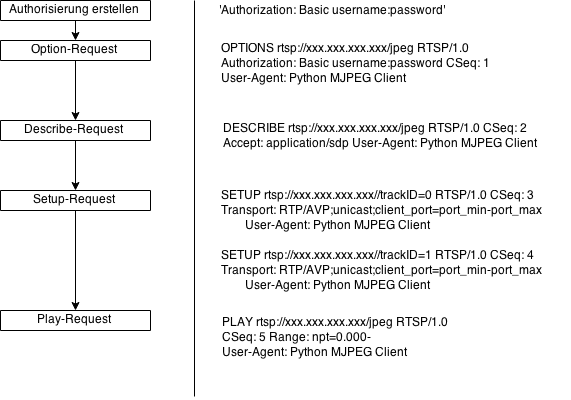
\includegraphics[width=\textwidth]{./data/RTSP.png}
	\caption{\label{fig:rtsprequest}RTSP Request Ablauf}
\end{minipage}
\end{figure}
\pagebreak

Nach dem PLAY-Request werden zwei neue UDP-Server-Instanzen generiert, die Daten des RTP-Streams auswerten (Audio / Video). Die Implementierung von Sergey Lalov liest an dieser Stelle die einzelnen Bilder eines MJPEG-Stream aus. Bei MJPEG werden in jedem Paket Einzelbilder gesendet\cite{mjpeg}. Dies führt dazu, dass aus einem einzelnen Paket ein Bild gewonnen werden kann.  \\
Die Kamera in diesem Projekt bietet im RTP-Stream den Videostream im Format H264\cite{h264} an. Da dieses Format verschiedene Arten der Komprimierung anwendet, ist nicht in jedem Paket ein einzelnes Bild enthalten. Die Rekonstruktion des Bildmaterials wäre somit sehr aufwändig (keine bestehende Library in Python). \\\\
Die Auswertung des RTP-Streams konnte somit nicht erfolgreich abgeschlossen werden.  

\subsection{Speicherung des Video-Streams mit FFmpeg}
Die Speicherung des Streams ist über eine externe Software möglich. Das Tool FFmpeg\cite{ffmpeg} ist eine Software-Lösung um Audio- und Videostreams aufzunehmen und zu konvertieren. Es bietet die Möglichkeit, einen Stream aufzuzeichnen und direkt im Anschluss in ein anderes Format zu Wandeln\cite{ffmpeg-tips}. 
\paragraph{Ablauf}
Im ersten Schritt wird mit FFmpeg der Stream eingelesen und pro Sekunde 3 Bilder daraus erzeugt. \\\\
\begin{lstlisting}[caption = Aufnahme mit FFmpeg und Konvertierung in Bilder (3FPS), language=python, frame=single, breaklines=true,columns=fullflexible, commentstyle=\color{gray}\upshape, captionpos=b]
ffmpeg -i rtsp://user:pw@$ip:554 -f image2 -vf fps=3 %03d.jpg -loglevel quiet
\end{lstlisting}
Diese Bilder werden in ein Verzeichnis gespeichert. Parallel dazu läuft ein Script, welches alle 60 Sekunden die ältesten Bilder aus diesem Verzeichnis löscht. Dadurch entsteht keine große Datenmenge, es sind nur die aktuellsten Bilder gespeichert. Wenn der Bewegungsmelder auslöst, werden die Bilder aus den letzten 10 Sekunden in ein weiteres Verzeichnis gelegt. Hierauf hat die iOS-App Zugriff über FTP.  \\
\begin{figure}[h]
\begin{minipage}{\textwidth}
	\centering
	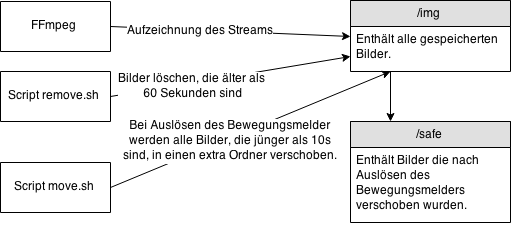
\includegraphics[width=\textwidth]{./data/ffmpeg.png}
	\caption{Ablauf der Aufzeichnung mit FFmpeg}
\end{minipage}
\end{figure}
\paragraph{Vorteil}
Ein großer Vorteil ist die hohe Variabilität der Konvertierung mit FFmpeg. Es kann nahezu jedes Format eingelesen werden und in variablen Frameraten ausgegeben werden. 
\paragraph{Nachteil}
Das Tool FFmpeg erzeugte eine sehr hohe Last auf dem System, da kontinuierlich eine Stream eingelesen wird. 

\subsection{Speicherung des Bild mittels Screenshot}

Ein weiterer Ansatz wäre das Aufrufen der Weboberfläche der Kamera und das Anfertigen eines Screenshots. Dieser könnte abgespeichert und auf einem FTP-Server bereitgestellt werden. \\
Hierfür ist es allerdings erforderlich, dass der Raspberry Pi eine grafische Ausgabe hat. In diesem Projekt soll er nur Serverfunktionalitäten haben. Als Work-Around bietet sich ein virtuelles Display an. Die Virtualisierung kann mittels dem Tool Xvfb\cite{xvfb} realisiert werden. Dieses bietet einen virtuellen Framebuffer, der vom System wie ein normales Display angesprochen werden kann. \\
Die Anfertigung eines Screenshots kann mit dem Tool Selenium\cite{selenium} erledigt werden. Das Tool Selenium dient zur Automatisierung von Browser-Aktivitäten und wird oft zum Testen von Webanwendungen verwendet. Selenium setzt ein Display vorraus, was durch Xvfb erfüllt wäre\cite{seleniumheadless}. Da Selenium nach Python portiert wurde, könnten die Screenshots direkt aus der Anwendung heraus erstellt werden. \\
Um diese Möglichkeit zu testen, wurde folgender Testcode implementiert:
\begin{lstlisting}[caption = Testcode - Aufnahme Screenshot mit Selenium, language=python, frame=single, breaklines=true,columns=fullflexible, commentstyle=\color{gray}\upshape, captionpos=b, numbers = left]
from selenium import webdriver
import time

start = time.time()
driver = webdriver.Firefox()
driver.get('user:password@ip_of_cam')
# get_screenshot_as_file() gibt das Bild als Binärdaten zurück
img = driver.get_screenshot_as_file()
driver.quit()
end = time.time()
print 'Benötigte Zeit:' + str(start - end)
\end{lstlisting}
Mehrere Messungen haben ergeben, dass das Aufnehmen des Screenshots rund 7 Sekunden dauert. Dies ist auf die geringe Rechenleistung des Raspberry Pi zurückzuführen. Außerdem wird mit Selenium ein vollständiger Browser gestartet, was zu einem enormen Overhead führt. \\
Die Durchführung dieser Methode macht aufgrund der hohen Verzögerung nur wenig Sinn. Eine Person die den Bewegungssensor auslöst ist längst aus dem Bild verschwunden, bis ein Screenshot aufgezeichnet wird.\\
\subsection{Speicherung des Bild mittels HTTP-Request} \label{subsec:kapitel-httprequest}

Die nächste Variante ist das Laden des Bildes aus dem HTML-Quelltext der Weboberfläche. Die Analyse des Quelltextes führt schnell zu dem Ergebnis, dass das angezeigte Bild mittels Javascript nachgeladen wird. Mit Python kann ohne weitere Probleme der Quelltext einer Webseite abgerufen werden: 
\begin{lstlisting}[caption = Testcode - HTTP-Request mit urllib2 in Python, language=python, frame=single, breaklines=true,columns=fullflexible, commentstyle=\color{gray}\upshape, captionpos=b, numbers = left]
import urllib2

response = urllib2.urlopen('http://ip_of_cam')
html = response.read()
\end{lstlisting}
Hier offenbart sich direkt das Problem, denn mit der Library urllib2\cite{urllib2} wird nur der HTML-Code abgerufen, ohne auf die Ausführung von Javascript zu warten\cite{urllib2-problem}. Somit kann über den Code zwar das Image-Objekt identifiziert werden, es enthält allerdings nur das Startbild. Mit dieser Version ist keine Lösung erreichbar. \\
Somit wird ein Framework benötigt, welches zuerst auf die vollständige Ausführen des Javascript-Codes wartet.
\begin{itemize}
	\item \textbf{Selenium}
	Hier könnte ebenfalls Selenium eingesetzt werden, welches einen Export des HTML-Code bietet. Allerdings würde auch hier der Zeitfaktor zu hoch sein. 
	\item \textbf{Scrapy}
	Dies ist ein open-source Framework, mit dem alle Informationen von Webseiten geladen werden könne. Die Installation auf dem Raspberry Pi war nicht erfolgreich.
\end{itemize}
Im nächsten Schritt wurde ein HTTP-Request an die URL gesendet, der im Javascript-Code als erstes aufgerufen wurde. Die Antwort enthielt ein aktuelles Frame der Kamera im Jpeg-Format. Das Abrufen dieses Bildes stellt in den meisten Sprachen keine große Schwierigkeit dar. \\
In Python wird das Bild mit dem Framework Requests\cite{requests} und StringIO\cite{stringio} geladen und in ein Bild umgewandelt. Dieses kann beliebig verarbeitet werden. 
\begin{lstlisting}[caption = Abrufen eines BIldes von einer URL in Python, language=python, frame=single, breaklines=true,columns=fullflexible, commentstyle=\color{gray}\upshape, captionpos=b, numbers = left]
from PIL import Image
import requests
from StringIO import StringIO

r = requests.get('http://user:password@ip:80/tmpfs/auto.jpg')
i = Image.open(StringIO(r.content))
i.save("path/to/safe/python_test.jpg")
\end{lstlisting}
Auch in Swift stellt dies kein Problem dar. Die Daten werden von der URL geladen und in ein UIImage\footnote{Objekt, welches diverse Arten von Bildern (z.B. jpg, png, tiff) speichern kann.}-Objekt gespeichert. 
\begin{lstlisting}[caption = Abrufen eines BIldes von einer URL in Swift, language=c++, frame=single, breaklines=true,columns=fullflexible, commentstyle=\color{gray}\upshape, captionpos=b, numbers = left]
let url = NSURL(string: camurl)
let data = NSData(contentsOfURL: url!)
let image : UIImage! = UIImage(data: data!)
\end{lstlisting}
Im Gegensatz zu der Implementierung mit FFmpeg muss nicht kontinuierlich ein Stream eingelesen werden, sondern es wird immer nur ein einzelnes Bild abgerufen, sobald der Bewegungsmelder auslöst. Es lassen sich somit zwei Ansichten realisieren:
\begin{itemize}
	\item \textbf{Archiv:} Bei Auslösen des Bewegungsmelders wird das aktuelle Bild abgerufen und auf einen FTP-Server gespeichert. Die Daten dieses Servers können in der iOS-App unter 'Archiv' abgerufen werden. 
	\item \textbf{Live:} In der iOS-App ist ein Live-View möglich. Dieser liest kein Video-Stream ein, sondern ruft in festgelegten Schritten ein Bild ab und aktualisiert die Ansicht. Um das Bild regelmäßig neu zu laden, wird ein NSTimer\footnote{Klasse, die nach festgelegten Zeitabschnitten Methoden aufruft.} genutzt. 
	\begin{lstlisting}[caption = NSTimer in Swift, language=c++, frame=single, breaklines=true,columns=fullflexible, commentstyle=\color{gray}\upshape, captionpos=b]
var timer = NSTimer.scheduledTimerWithTimeInterval(0.5, target: self, selector: Selector("loadImageView"), userInfo: nil, repeats: true)
	\end{lstlisting}
\end{itemize}
\pagebreak
\begin{figure}[h]
	\begin{minipage}{0.9\textwidth}
		\centering
		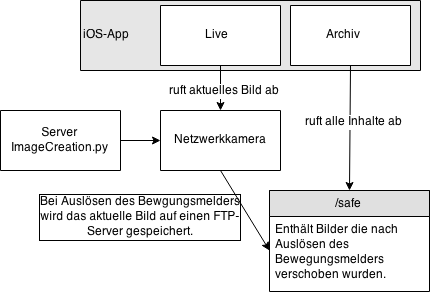
\includegraphics[width=\textwidth]{./data/httprequest.png}
		\caption{Abrufen des Bildes über HTTP-Request}
	\end{minipage}
\end{figure}

\paragraph{Fazit} 
Das Speichern des Kamerabildes mittels Screenshot und RTSP-Protokoll sind fehlgeschlagen. Die Aufnahme mit FFmpeg funktioniert gut, benötigt allerdings sehr viele System-Ressourcen. Somit ist der gewählte Weg in diesem Projekt das Abspeichern des Bildes über einen HTTP-Request. Diese Lösung ist gut in Python und Swift umzusetzen. 


\section{Anwendungsstruktur}
\subsection{Klassen und ihre Funktionen}

\begin{figure}[h]
	\begin{minipage}{\textwidth}
		\centering
		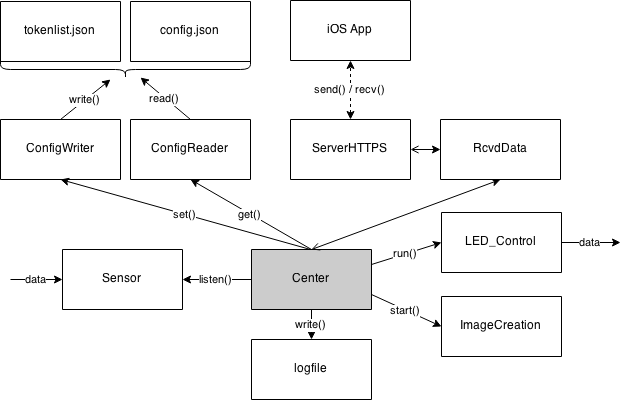
\includegraphics[width=\textwidth]{./data/ApplicationConcept.png}
		\caption{Anwendungsstruktur Server-Anwendung}
	\end{minipage}
\end{figure}

\begin{itemize}
\item Center\\
Die Klasse 'Center' stellt die zentrale Stelle in der Anwendung dar, an der alle Informationen zusammen laufen und verwaltet werden.
\item ServerHTTPS\\
Hier läuft der Webserver, welcher Nachrichten empfängt und sendet. Empfangene Nachrichten werden an die Klasse 'RcvdData' übergeben.
\item RcvdData\\
Hier werden die empfangenen Nachrichten ausgewertet und entsprechende Antworten generiert. Diese werden an den Webserver zurück gegeben und abgesendet. Die Prüfung der Korrektheit der einzelnen Protokollbestandteile findet ebenfalls hier statt. Wenn alle Überprüfungen erfolgreich sind, werden die Befehle an 'Center' weiter gegeben und dort ausgeführt.
\item Sensor\\
In der Klasse 'Sensor' werden die einzelnen Bewegungssensoren überwacht. Falls eine Bewegung detektiert wird, so werden in 'Center' die notwendigen Methoden aufgerufen um die LEDs an- oder auszuschalten.
\item LED-Control\\
Die Klasse 'LED\_Control' verwaltet die eingerichteten LEDs und steuert diese. Hier werden auch die möglichen Effekte gesteuert. Die Methoden in dieser Klasse werden aus der Klasse 'Center' aufgerufen. Ein Zugriff in die andere Richtung ist nicht möglich.
\item ConfigReader / ConfigWriter\
Diese beiden Klassen bieten die Möglichkeit die Konfigurationsdatei config.json zu lesen und zu schreiben. In der Konfiguration werden Informationen wie Anzahl der LEDs, Passworthash oder Adresse der Netzwerkkamera abgespeichert. Die Konfigurationsdatei wird beim Installationsvorgang erstellt.
\item ImageCreation\\
Abrufen von Bildmaterial von der Netzwerkkamera oder vom Server findet ausschließlich über die Klasse 'ImageCreation' statt. Die Klasse ruft die Informationen ab und filtert das Bildmaterial. Außerdem ist sie fähig, die gespeicherten Bilder zu Verwalten und das FTP-Verzeichnis zu mounten.
\item Logfile\\
Im Logfile werden unter anderem auftretende Fehler gespeichert.
\end{itemize}

\subsection{Auswertung empfangener Daten}
Da die Daten anhand des ausgearbeiteten Protokolls übertragen werden, können sie als String sehr einfach an den ":" aufgesplittet werden. Im Anschluss werden sie einzelnen Variablen zugewissen (bessere Lesbarkeit des Codes). Bevor das 'Control'-Feld ausgewertet wird, muss der Hashwert der Übertragung und die Authentifizierung geprüft werden. \\\\
\textbf{RecvdData.py Auswertung} 
\begin{lstlisting}[caption=Auswertung der empfangenen Daten (RcvdData.py), language=python, frame=single, breaklines=true,columns=fullflexible, commentstyle=\color{gray}\upshape, captionpos=b, numbers = left]
def dataReceived(self, data):
 # Protokoll: user:pw:control:ledNo:rangeStart:rangeEnd:red:green:blue:modus:effectcode:config:hashv
 # Beispiel: admin:w:X00:1:0:0:10:10:10:0:0:w-w:58acb7acccce58ffa8b953b12b5a7702bd42dae441c1ad85057fa70b
 # Ermoeglicht Zuweisung von Farben und Effekten
 # Ermöglicht Abruf von aktuellem Status des Systems und der LEDs
 #
 # Ankommende String bei ":" aufsplitten und in Array a[] Speichern:
 a = data.split(':')
 print a
 if len(a) > 1:
 user =         a[0]
 pw =         a[1]
 control =     a[2]
 ledNo =     a[3]
 rangeStart = a[4]
 rangeEnd =     a[5]
 red =         a[6]
 green =     a[7]
 blue =         a[8]
 modus =     a[9]
 effectcode = a[10]
 config = a[11]
 hashv = a[12]
 data = user + pw + control + ledNo + rangeStart + rangeEnd + red + green + blue + modus + effectcode + config
 data = data.rstrip('\n')
 data = data.rstrip('\r')
 if (self.checkAuthentification(user, pw) & self.checkTransmissionData(data, hashv)):
   if control == 'X00':
     ## Alle LEDs ausschalten
     center.clearPixel()
   elif control == 'X01':
     ## Eine LED anschalten
     self.lightUpOneLED(int(ledNo), int(red), int(green), int(blue))
   elif control == 'X02':
     ## LED Bereich anschalten
     self.lightUpLEDRange(int(rangeStart), int(rangeEnd), int(red), int(green), int(blue))
   elif control == 'X03':
     ## Eine Farbe für alle LED
     self.lightUpAllLED(int(red), int(green), int(blue))
   elif control == 'X04':
     ## Effekt alle LEDs
     self.effectLED(effectcode)
   elif control == 'X05':
     ## Modus des Systems
     self.changeModus(int(modus))
   elif control == 'X06':
     ## Systemstatus als JSON an den Client
     return self.sendStatus()
   elif control == 'X07':
     ## Status der einzelnen LEDs senden
     return self.sendLEDStatus()
   elif control == 'X08':
     ## Konfiguration ändern
     self.changeConfiguration(config)
   elif control == 'X09':
     ## Login
     return "LOGIN:TRUE"
   else:
     print center.writeLog('Übertragung fehlerhaft')
\end{lstlisting}
Die komplette Klasse ist einsehbar unter: \url{https://github.com/hoedding/Studienarbeit-Anwendung/blob/master/RaspberryPI/RecvdData.py} \\\\ 

\textbf{RecvdData.py gesamt} 
\begin{lstlisting}[caption =Implementierung des Nachrichten-Verarbeitung in Python, language=python, frame=single, breaklines=true,columns=fullflexible, commentstyle=\color{gray}\upshape, captionpos=b, numbers = left]
#!/usr/bin/python
# -*- coding: utf-8 -*-
#######################
# Author: Timo Höting                          #
# Mail: mail[at]timohoeting.de                 #
#######################

import hashlib
from ConfigReader import *
import threading

class RecvdData(threading.Thread):
def __init__(self, c):
threading.Thread.__init__(self)
global center
center = c

def dataReceived(self, data):
# Aufteilung der übertragenenen Daten

def changeModus(self, modus):
# Modus des Systems ändern.

def lightUpOneLED(self, ledNo, red, green, blue):
# Eine einzelne LED mit den o.g. RGB-Werten dauerhaft anschalten

def lightUpLEDRange(self, rangeStart, rangeEnd, red, green, blue):
# Einen Bereich von LEDs mit den o.g. RGB-Werten
# dauerhaft einschalten
# Bereich muss ueberprueft werden mit checkRange()

def lightUpAllLED(self, red, green, blue):
# Alle LEDs mit den o.g. RGB-Werten
# dauerhaft einschalten
# Bereich muss ueberprueft werden mit checkRange()

def effectLED(self, code):
# Effekte auf einer LED aktivieren

def checkRange(self, ledNo):
# Ueberprueft ob die uebergeben LED-Nummer ueberhaupt im
# gueltigen Bereich liegt
# Es wird der Eintrag 'number' aus dem Config-File geladen

def checkColorRange(self, color):
# Überprüfung ob Farbwert im gültigen Bereich liegt

def checkAuthentification(self, user, pw):
# Authentifizierung überprüfen
# Eingabewert ist das Passwort aus der Übertragung
# Dieses wird gehasht und mit dem in der Konfiguration gespeicherten
# Hashwert verglichen

def checkTransmissionData(self, data, check):
# Korrektheit der Übertragung mittels Hashvergleich feststellen
# Eingabewert sind die gesamten Daten der Übertragung

def sendStatus(self):
# Status des Systems senden

def sendLEDStatus(self):
# Farbwerte aller einzelnen LEDs senden

def changeConfiguration(self, config):
# Konfiguration der Anwendung ändern
\end{lstlisting}
Der vollständige Code ist unter \url{https://github.com/hoedding/Studienarbeit-Anwendung/blob/master/RaspberryPI/RecvdData.py} einsehbar.



\subsection{Konfiguration}
\paragraph{Konfigurations-Datei}
Die Informationen die zum Betrieb notwendig sind, werden in JSON-Format gespeichert.
\begin{lstlisting}[caption=Konfigurationsdatei config.json, language=xml, frame=single, breaklines=true,columns=fullflexible, commentstyle=\color{gray}\upshape, captionpos=b, numbers = left]
{
 "username": "",
 "ledport":"", 
 "motionport2": "", 
 "motionport1": "", 
 "cam_url": "", 
 "pw": "", 
 "ledcount": "", 
 "timeperiod": "", 
 "camavaible": "", 
 "ftp_host":"", 
 "ftp_directory":"", 
 "ftp_user":"", 
 "ftp_pw":"", 
 "cam_user":"", 
 "cam_pw":"", 
 "cam_host":"",
 "cam_dir":""
}
\end{lstlisting}
Einige dieser Informationen können für die Synchronisation des Clients gesendet werden.
\begin{lstlisting}[caption=Senden von Konfigurationsinformationen an den Client, language=xml, frame=single, breaklines=true,columns=fullflexible, commentstyle=\color{gray}\upshape, captionpos=b, numbers = left]
def sendStatus(self):
	 # Status des Systems senden
	 reader = ConfigReader()
	 message = 'STATUS:{"ledcount":"' + reader.getValue("ledcount") + '","motionport1":"' + reader.getValue("motionport1") + '","motionport2":"' + reader.getValue("motionport2") + '","camavaible":"'
	 message = message + reader.getValue("camavaible") + '","timeperiod":"' + reader.getValue("timeperiod") + '","ftpdir":"' + reader.getValue("ftp_directory") + '","ftphost":"' + reader.getValue("ftp_host")
	 message = message + '","camuser":"' + reader.getValue("cam_user") + '","ftpuser":"' + reader.getValue("ftp_user") + '","ftppw":"' + reader.getValue("ftp_pw") + '","camhost":"' + reader.getValue("cam_host") + '"}'
	 return str(message)
\end{lstlisting}

\paragraph{Status der LED} Es ist möglich der Status der einzelnen LEDs abzurufen. Hierfür wird ein JSON-Objekt generiert, welches die einzelnen Farben als 24Bit RGB-Werte enthält.
\begin{lstlisting}[caption=Status der LEDs an Client senden, language=xml, frame=single, breaklines=true,columns=fullflexible, commentstyle=\color{gray}\upshape, captionpos=b, numbers = left]
def getLEDStatusAsJson(self):
	led_values = led.getLedAsArray()
	data = 'LED:{"led": ['
	count = 0
	if len(led_values) > 0:
	for i in range(0, len(led_values)-1):
	data = data + '{"l":"' + str(led_values[i]) + '"},'
	count = count + 1
	data = data + '{"l":"' + str(led_values[len(led_values)-1]) + '"}]}'
	count = count + 1
	return data
  
\end{lstlisting}

\paragraph{Lesen und Schreiben der Konfiguration}  Um die Konfiguration lesend und schreiben bearbeiten zu können wird ein ConfigReader und ein ConfigWriter implementiert. Bei jeder neuen Verbindung der iOS-App zum Server wird das Token für die Notification übertragen. Diese wird, falls noch nicht vorhanden, in die Datei tokenlist.json eingetragen. Das neue Passwort muss vor dem Abspeichern noch in einen Hash-Wert umgewandelt werde. 
\begin{lstlisting}[caption=ConfigReader / ConfigWriter, language=xml, frame=single, breaklines=true,columns=fullflexible, commentstyle=\color{gray}\upshape, captionpos=b, numbers = left]
class ConfigReader():
	def getValue(self, key):
		if key == "token":
			return self.getToken()
			data = open('config.json')
			jdata = json.load(data)
			return jdata[key]

	def getToken(self):
		data = open('tokenlist.json')
		jdata = json.load(data)
		return jdata["token"]

class ConfigWriter():
	def changeConfig(self, key, value):
		jsonFile = open("config.json", "r")
		jdata = json.load(jsonFile)
		jsonFile.close()
		jdata[key] = value
		jsonFile = open("config.json", "w+")
		jsonFile.write(json.dumps(jdata))
		jsonFile.close()

	def changePassword(self, value):
		hashpw = hashlib.sha224(value).hexdigest()
		jsonFile = open("config.json", "r")
		jdata = json.load(jsonFile)
		jsonFile.close()
		jdata["pw"] = hashpw
		jsonFile = open("config.json", "w+")
		jsonFile.write(json.dumps(jdata))
		jsonFile.close()
		
	def addNewToken(self, token):
		jsonFile = open("tokenlist.json", "r")
		jdata = json.load(jsonFile)
		jsonFile.close()
		tokens = jdata['token']
		for element in tokens:
		if element['t'] == token:
			return
		jdata['token'].append({"t":token})
		jsonFile = open("tokenlist.json", "w+")
		jsonFile.write(json.dumps(jdata))
		jsonFile.close()
\end{lstlisting}

\subsection{Apple Push Notification} 
\paragraph{Eigenschaften}
Die Notifications können von nahezu jedem System an den Apple-Server gesendet werden. Dieser gibt Rückmeldung, ob das Format der Notification korrekt ist und sendet sie an das jeweilige Device. Falls das Gerät nicht verfügbar ist, wird sie eine gewisse Zeit zwischengespeichert, bevor sie verworfen wird. \\
Jede Notification enthält Darstellungseigenschaften für den Client und einen Payload mit der Größe 2kb (vor iOS 8 sind es 256Bytes). Die Daten werden in Form von JSON übertragen.\\
Es können zum Beispiel folgende Informationen übergeben werden: 
\begin{itemize}
	\item Titel der Meldung
	\item Inhal der Meldung
	\item Nummer für das App-Icon
	\item Der abzuspielende Sound
\end{itemize}
\textbf{Implementierung}\\
Für die Implementierung wird die Library PyAPNs https://pypi.python.org/pypi/apns/ eingesetzt. Diese bietet alle Möglichkeiten, auf einfach Art und Weise, Notifications zu senden. \\
Bei der Initialisierung werden die gespeicherten Tokens aus der Datei tokenlist.json geladen. Im Anschluss kann über die push()-Methode die Notification an alle Geräte gesendet werden. 
\begin{lstlisting}[caption=ConfigReader / ConfigWriter, language=xml, frame=single, breaklines=true,columns=fullflexible, commentstyle=\color{gray}\upshape, captionpos=b, numbers = left]
#!/usr/bin/python
# -*- coding: utf-8 -*-
#######################
# Author: Timo Höting						  #
# Mail: mail[at]timohoeting.de				 #
#######################

import sys, time
from apns import APNs, Frame, Payload
from ConfigReader import *

class ApplePush():
	def __init__(self):
		reader = ConfigReader()
		tokenlist = reader.getValue("token")
		global token
		token = []
		# Alle Tokens werden aus der Liste geladen
		for i in tokenlist:
			token.append(i['t'])

	# Das Apple-Device bekommt eine Message gepusht
	def push(self, message):
		# Developer Zertifikat für iOS Push Benachrichtigung
		apns = APNs(use_sandbox=True, cert_file='certs/Studienarbeit-APN.crt.pem', key_file='certs/Studienarbeit-APN.key.pem')
		payload = Payload(alert="Bewegung erkannt!", sound="default", badge=1)
		for i in token:
			apns.gateway_server.send_notification(i, payload)
\end{lstlisting}


\subsection{Unit-Test}
In Python ist es möglich Unit-Tests zu schreiben. Mit diesen wird hauptsächlich die Initialisierung der einzelnen Klassen geprüft. So kann schnell herausgefunden werden, ob in diesen Implementierungsfehler vorliegen. Außerdem werden ConfigReader und ConfigWriter getestet. \\
Eine Ausgabe sieht so aus:

\begin{lstlisting}[caption=Ausgabe der Klasse UNIT\_Test, language=python, frame=single, breaklines=true,columns=fullflexible, commentstyle=\color{gray}\upshape, captionpos=b, numbers = left]
root@raspberrypi:/home/timo/Studienarbeit# python UNIT_Test.py 
test_Center (__main__.TestSequenceFunctions) ... ok
test_Effects (__main__.TestSequenceFunctions) ... ok
test_LEDControl (__main__.TestSequenceFunctions) ... ok
test_Sensor (__main__.TestSequenceFunctions) ... ok
test_Server (__main__.TestSequenceFunctions) ... ok
test_Status (__main__.TestSequenceFunctions) ... ok
test_camAdress_MUST_FAIL (__main__.TestSequenceFunctions) ... FAIL
test_camAvaible (__main__.TestSequenceFunctions) ... ok
test_getHashPass (__main__.TestSequenceFunctions) ... ok
test_getMotionPin1 (__main__.TestSequenceFunctions) ... ok
test_getNumberOfLED (__main__.TestSequenceFunctions) ... ok

=============================================
FAIL: test_camAdress_MUST_FAIL (__main__.TestSequenceFunctions)
--------------------------------------------
Traceback (most recent call last):
  File "UNIT_Test.py", line 67, in test_camAdress_MUST_FAIL
    self.assertEqual(resultTest, resultCorrect)
AssertionError: '192.168.2.205' != '123'

--------------------------------------------
Ran 11 tests in 1.873s
\end{lstlisting}
\subsection{Threads}

\begin{wrapfigure}{l}{0.4\textwidth}
	\vspace{-20pt}
	\begin{center}
		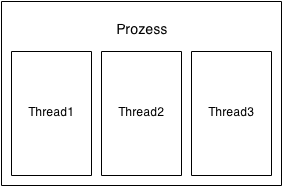
\includegraphics[width=0.3\textwidth]{./data/Threads.png}
	\end{center}
	\vspace{-20pt}
	\caption{Prozess und Threads}
	\vspace{-10pt}
\end{wrapfigure}

\paragraph{Problem}  Die Server-Klasse und Sensor-Klasse befinden sich in einer Endlosschleife, da sie dauerhaft auf eine Eingabe warten. Beim Server sind dies Empfangene Daten und beim Sensor Bewegungssignale. Würden alle Klassen in einem Thread ablaufen, so würde nur eine Klasse gestartet werden und der Anwendungsablauf in dieser bleiben. 
\paragraph{Lösung}  Die beiden oben genannten Klassen, sowie weitere Klassen wie die LED-Steuerung, werden in eigene Threads ausgelagert. Threads sind Unterprozesse im Hauptprozess, die es ermöglichen mehrere Aufgaben in einem Programm gleichzeitig abzuarbeiten. Zwischen den einzelnen Threads kann Datenaustausch statt finden und es ist möglich übergreifende Funktionen aufzurufen. \\
Zur Implementierung wird das Modul 'threading' genutzt. Eine Klasse, die in einem Thread gestartet werden soll, benötigt eine init- und eine run-Methode.
\paragraph{Beispielcode}
Für eine Funktionsdarstellung der Threads mit Python werden drei Klassen angelegt, eine zur Steuerung und zwei, die in einem Thread laufen sollen. \\
Die Klasse 'Testcenter' initialisiert die Klassen als Threads und startet diese.
\begin{lstlisting}[caption=Klasse Testcenter, language=python, frame=single, breaklines=true,columns=fullflexible, commentstyle=\color{gray}\upshape, captionpos=b, numbers = left]
#!/usr/bin/python
# -*- coding: utf-8 -*-
##############################
# Author: Timo Höting                        #
# Mail: mail[at]timohoeting.de            #
##############################
import threading
from TestThread import *
from TestThread1 import *

class TestCenter():
    def newThread(self):
        global testthread
        global testthread1
        testthread = TestThread('thread0', self)
        testthread1 = TestThread1('thread1', self)
        testthread.start()
        testthread1.start()

    def dosth(self):
        print 'dosth'

    def dosth2(self):
        print 'dosth2'

    def dosth3(self):
        testthread1.calledFromMain('-dosth3')

if __name__ == "__main__":
    newThread = TestCenter()
    newThread.newThread()
\end{lstlisting}
Die beiden TestThread-Klassen enthalten beide eine init- und eine run-Methode. Die Klasse Thread1 enthält zusätzlich noch eine Methode die von anderen Klassen ausführbar ist. 
\begin{lstlisting}[caption=Klasse TestThread1, language=python, frame=single, breaklines=true,columns=fullflexible, commentstyle=\color{gray}\upshape, captionpos=b, numbers = left]
#!/usr/bin/python
# -*- coding: utf-8 -*-
##############################
# Author: Timo Höting                        #
# Mail: mail[at]timohoeting.de            #
##############################

import threading
import time
import datetime

class TestThread1(threading.Thread):
    def __init__(self,ms,c):
        threading.Thread.__init__(self)
        global center
        center = c
        global message
        message = ms

    def run(self):
        print message
        center.dosth2()

    def calledFromMain(self, message):
        print  'calledFromMain' + message
\end{lstlisting}
Die init()-Methoden werden bei der Erzeugung des Threads aufgerufen und die run()-Methode wenn er gestartet wird. Danach können die Methoden wie bei normalen Methodenaufrufen benutzt werden. 

\paragraph{Cleanup}
Um die einzelnen Threads korrekt zu beenden sind Methoden zum Aufräumen notwendig. Dies ist vor allem bei Threads wichtig, die sich in einer Endlosschleife befinden oder Server-Anwendung beherbergen. 
\begin{itemize}
	\item \textbf{Webserver:} Im Thread des Twisted-Webservers wird eine Methode implementiert, die den Server korrekt herrunterfährt. Somit wird auch der reservierte Port frei gegeben. 
	\item \textbf{Sensorauswertung:} Die Sensorauswertung befindet sich in einer Endlosschleife, welche beendet werden muss. Die Schleife wird abhängig einer Variable implementiert. In der Cleanup-Methode wird diese Variable auf false gesetzt. 
	\item \textbf{LED-Ansteuerung:} Beim Stoppen der Anwendung müssen alle LEDs ausgeschaltet werden. 
	\item \textbf{Kameraaufnahme:} Da zu Beginn der Aufnahme ein FTP-Verzeichnis gemountet wird, muss dieses am Ende frei gegeben werden. Andernfalls können beim neuen Verbinden Fehler entstehen.
\end{itemize}
// TODO Grafik über Zusammenspiel
\section{Konfiguration und Installation}
\subsection{Konfiguration}
\subsection{Installation}

\section{iOS App}
\subsection{Konzept}
\subsection{...}
\subsection{...}

\chapter{Praktische Umsetzung}

\chapter{Kostenaufstellung}

\chapter{Fazit}

\pagebreak
\section{Abbildungsverzeichnis}

\listoffigures


\clearpage
\addcontentsline{toc}{chapter}{\lstlistlistingname}

\lstlistoflistings


\begin{thebibliography}{xxxxxxxxxxxxxxxxxxx}
 \bibitem[I.]{eventbased}"'SWR Info - Zahlen, Daten, Fakten über den SWR"', \url{http://www.swr.de/unternehmen/unternehmen/kennzahlen/kennzahlen-organisation/-/id=12213420/did=12302978/nid=12213420/eqq46v/index.html}, 13.12.2013
%\bibitem[Thema]{Bezeichner}"'Überschrift"', \url{LINK}, Datum
%\cite{Bezeichner}
\end{thebibliography}









 \end{document}

 